% Interesting trick to instead make the chapter number the letter C for this appendix.
\begingroup
\renewcommand\thechapter{D}
\titleformat{\chapter}[display]
{\normalfont\huge\bfseries}{}{20pt}{\Huge}
\setcounter{section}{0} % Set the section counter back to 0 so that Appendix C doesn't interfere.

\chapter*{Appendix D - Additional techniques}
\addcontentsline{toc}{chapter}{Appendix D - Additional techniques}
\markboth{Appendix D}{}

To enhance the performance of the models, a second iteration of each model was created.
These models implemented stratified cross-validation and hyperparameter tuning to improve 
the evaluation metrics, and therefore predictive capabilities, of each model.

\section{Cross-Validation}
\subsection{Definition}
Cross-validation is a technique used in machine learning to evaluate a model's performance on unseen data. It involves 
partitioning the dataset into subsets, using some subsets for training and others for validation, and repeating this
process multiple times with different partitions. This helps assess how well the model generalizes to new data and can
detect issues like overfitting. This is typically done using KFold.

\begin{figure}[H]
    \centering 
    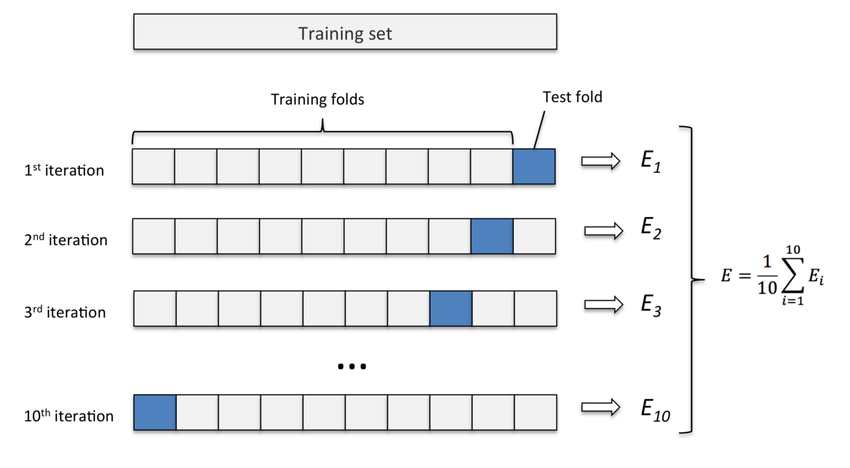
\includegraphics[width=\linewidth]{ModelDev/Iteration2/KFoldExample.png}
    \caption{A visual representation of KFold cross-validation \autocite{rosaen_scikit-learn_nodate}.}
    \label{fig:KFExample}
\end{figure}

\para However, KFold does not account for class imbalance, which means that the sets it chooses may have 
differing levels of balance across the target class. Even in balanced datasets, this can still occur if the 
data has been shuffled as the set chosen may still contain fewer rows of one class than the other. This is 
solved by stratified cross-validation.

\begin{figure}[H]
    \centering 
    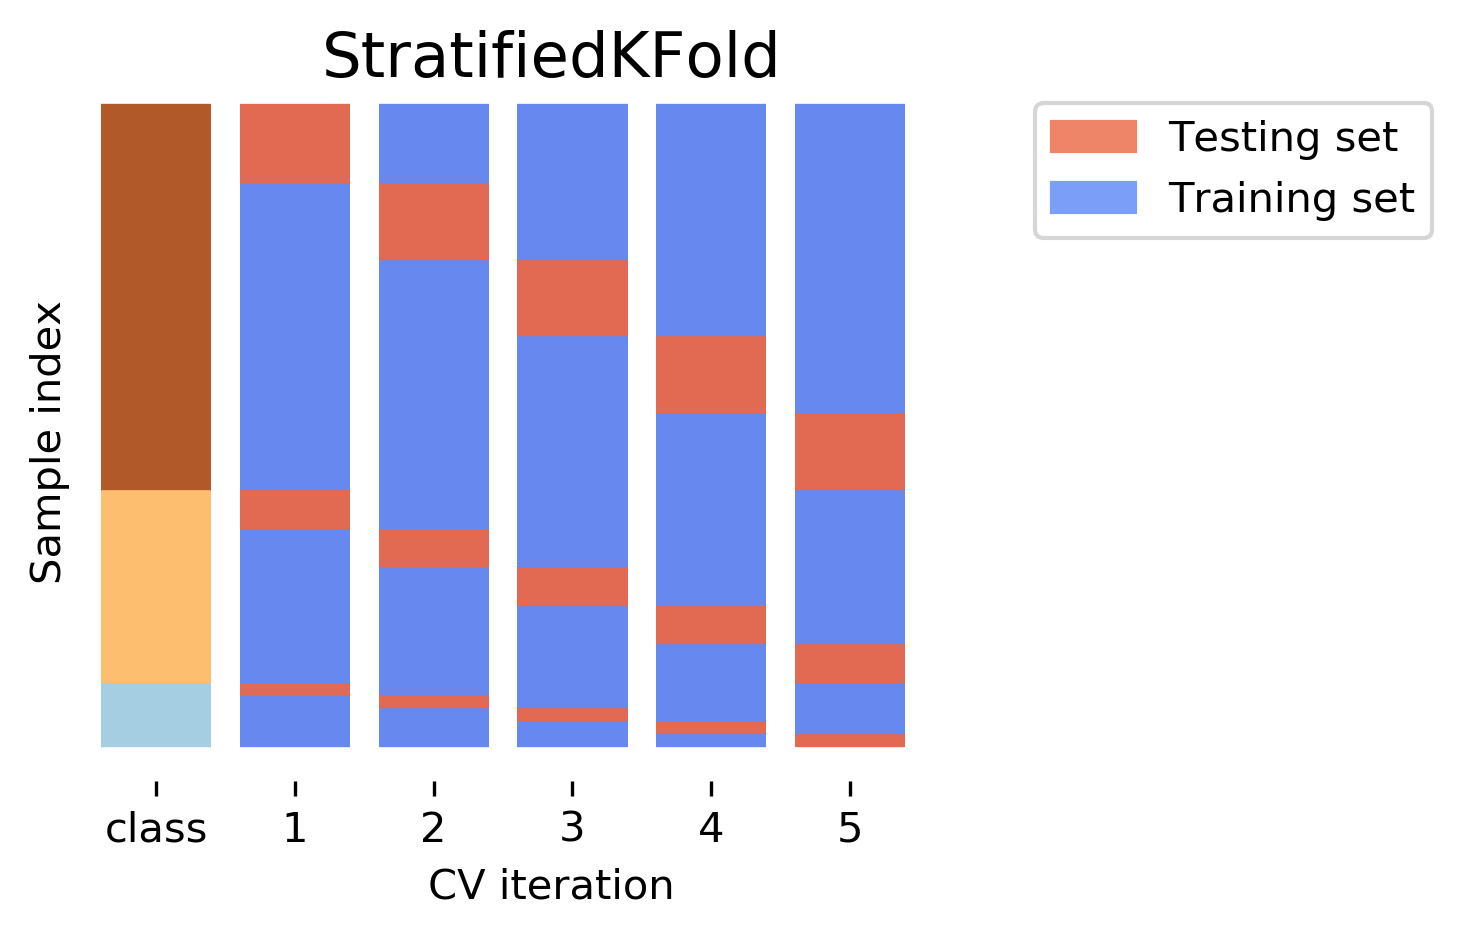
\includegraphics[width=\linewidth]{ModelDev/Iteration2/StratifiedKFoldExample.png}
    \caption{A visual representation of StratifiedKFold cross-validation \autocite{muller_data_nodate}.}
    \label{fig:SKFExample}
\end{figure}

\para Stratified cross-validation is a variant that ensures each fold maintains the same proportion of samples for each 
target class. This is particularly useful for imbalanced datasets, as it helps maintain the class
distribution across all folds, providing a more reliable estimate of the model's performance across various subsets of data, 
though it still is helpful even in balanced datasets. This dataset was balanced using SMOTE, though a stratified approach 
can still be beneficial for it.

\para Another key topic with KFold and StratifiedKFold is the amount of folds to use. As with train/test splits, there 
does not appear to be a definitive answer to the amount of folds to use in every dataset. However, previous literature 
on model development with this datasets such as that of \textcite{zou_construction_2024}'s used ten folds and achieved 
strong results, showcasing that this number of folds can work well with this data. Therefore, this project will also use ten folds.

\pagebreak 

\subsection{Application}
The new iterations use 10 fold stratified cross-validation through StratifiedKFold as shown in Figure \ref{fig:SKFCode}. 

\begin{figure}[H]
    \centering 
    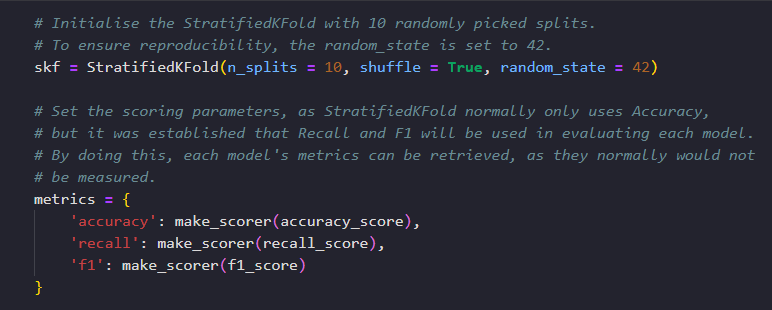
\includegraphics[width=\linewidth]{ModelDev/Iteration2/SKF+Metrics.png}
    \caption{The code used to instantiate a 10-fold StratifiedKFold.}
    \label{fig:SKFCode}
\end{figure}

\para The method used to perform hyperparameter tuning will take the SKF object as a parameter, so its implementation 
is displayed in Section \ref{ASec:HyperparameterApplication}.


\section{Hyperparameter tuning}
\subsection{Definition}
Hyperparameter tuning refers to the configuration of parameters passed to a machine learning algorithm to alter its 
functionality. It is performed to maximise the predictive ability of a model, as models can have drastically different 
results depending on the parameters they were trained with. Some examples of parameters include the amount of decision trees 
(n\_estimators) in a Random Forest, or the amount of neighbours (n\_neighbors) in KNN.

\para Hyperparameter tuning can be performed manually by changing the parameters with each individual run of the model after evaluating 
its metrics, or automatically using Scikit-Learn functionality such as GridSearchCV. Automatic methods like GridSearchCV can be much faster than 
manual hyperparameter tuning.
% Insufficient detail, add source.

\para GridSearchCV is supplied with a dictionary of parameters, known as the parameter grid. It will then exhaustively evaluate a model
using every combination of parameters assigned in the parameter grid. This requires the fitting and training of a new model for every single 
combination, which is extremely computationally intensive in terms of processing power and memory usage. After this is completed, the GridSearchCV 
object will return the best model based on the metrics it achieved.

\subsection{Application}\label{ASec:HyperparameterApplication}

\begin{figure}[H]
    \centering 
    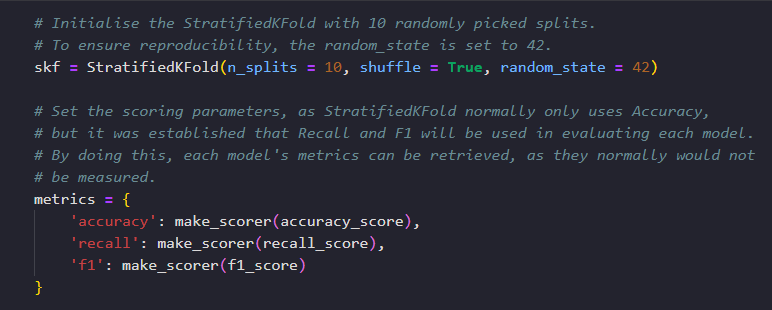
\includegraphics[width=\linewidth]{ModelDev/Iteration2/SKF+Metrics.png}
    \caption{The code used to instantiate a 10-fold StratifiedKFold.}
    \label{fig:SKFCode}
\end{figure}